\usepackage[T1]{fontenc}
\usepackage[utf8]{inputenc}
\usepackage{graphicx}

%!TEX ROOT=../diploma-thesis.tex

\chapter{Analýza}\label{ch:analyza}

Tato kapitola analyzuje problematiku byznysových pravidel v informačních systémech.
Dále detailně popisuje architekturu orientovanou na služby, včetně jejího historického
vývoje a moderního trendu v podobě microservices. Na základě toho kapitola popisuje nedostatky
při řešení průřezových problémů v těchto architekturách, s důrazem na byznysová pravidla.
V závěru kapitoly jsou identifikovány požadavky, které by měl splňovat framework,
jež bude výstupem této diplomové práce.

\section{Byznysová pravidla}

Informační systémy (IS) mají za úkol ulehčit, automatizovat či poskytovat podporu pro
byznysové procesy společností, které je využívají. Tyto procesy jsou tedy stěžejním
prvkem IS. Systém má také za úkol uchovávat a spravovat data společnosti
a měl by zaručit, že nedojde k jejich poškození či narušení jejich integrity.
Byznysové procesy, potažmo byznysové operace, proto musejí
podléhat jasně definovaným byznysovým pravidlům, která zajišťují konzistenci dat informačního
systému a také zabraňují nepovoleným operacím~\cite{cemus2015automated}.

Byznysová pravidla dělíme do tří skupin~\cite{cemus2014aspect}:
\begin{description}
    \item [Bezkontextová pravidla] jsou validační pravidla, která musejí být obecně platná
    v každé operaci, jinak by mohlo dojít k porušení integrity dat systému. Příkladem může
    být pravidlo \uv{\textit{Adresa uživatele je platnou e-mailovou adresou}}.
    \item [Kontextová pravidla] jsou pravidla, která musejí být zohledněna v daném kontextu
    byznysové operace, například \uv{\textit{Při přidání produktu do košíku nesmí součet položek
    v košíku přesahovat částku milion korun}}
    \item [Průřezová pravidla] jsou parametrizována stavem systému nebo uživatelského účtu a mají
    dopad na velkou část systému. Uvažme pravidlo \uv{\textit{V systému nesmí probíhat žádné změny po
    dobu učetní uzávěrky}}.
\end{description}

Dále také rozlišujeme dva typy byznysových pravidel, a těmi jsou \textit{preconditions}
a \textit{post-conditions}~\cite{cemus2015automated}.

\subsection{Precondition}

Aby mohla být byznysová operace vykonána, musejí
být splněny předem definované podmínky, neboli předpoklady,
které nazýváme \textit{preconditions}. Pokud alespoň jedna z podmínek
není splněna, byznysová operace nemůže proběhnout.

Pro lepší ilustraci uveďme příklad: aby mohla být provedena
registrace uživatele s danou emailovou adresu, musí být splněna
podmínka, že uživatel vyplnil svojí emailovou adresu a zároveň
dosud v systému neexistuje žádný uživatel se stejnou emailovou adresou.

\subsection{Post-condition}

Na byznysovou operaci mohou být kladeny požadavky, které
musejí být splněny po jejím úspěšném vykonání. Příkladem
může být anonymizace uživatelů při vytváření statistického
reportu e-commerce společnosti – po vygenerování reportu
post-condition zajistí, že z něj budou smazány veškeré citlivé údaje.
Dalším případem může být filtrování výstupu byznysové operace.
Například při výpisu objednávek pro zákazníka se chceme ujistit, že
všechny vypsané objednávky patří danému zákazníkovi.

\subsection{Reprezentace byznysového pravidla}

Existuje několik možností, jak zachytit a reprezentovat byznysová pravidla~\cite{cemus2015automated}.
Nejběžnější a nejpoužívanější metodou je jejich zachycení v programovacím
jazyce. Tato metoda je snadná, protože se programátor může použít stejný jazyk
pro popis pravidel stejně jako pro popis celého systému. Bohužel, tato metoda
nám nedává příliš možností, kterými můžeme provést inspekci a extrakci pravidel.
Další, pokročilejší metodou, je zápis pravidel pomocí meta-instrukcí, například anotací,
nebo tzv.\textit{Expression Language} (EL). Tato metoda poskytuje dobrou možnost inspekce,
ale zpravidla není typově bezpečná a může snáze způsobovat chyby v programu.
Poslední, nejpokročilejší metodou, je zápis pomocí doménově specifických jazyků.
Ty jsou snadno srozumitelné nejen pro programátory, ale i pro doménové experty.
Nevyžadují inspekci a mohou být typově bezpečné. Mezi jejich nevýhody ale patří vysoká
počáteční investice v podobě návrhu takového jazyka a nutnost jeho kompilace nebo
interpretace.

\subsection{Byznysový kontext}

Informační systém zpravidla implementuje více byznysových procesů, které se vážou
na jeden či více uživatelských scénářů. Uživatelský scénář se pak dělí na jednotlivé
kroky, například zaslání potvrzovacího e-mailu k objednávce, či uložení objednávky
do databáze. Tyto kroky nazýváme \textit{byznysové operace} – tedy operace, které mají
byznysovou hodnotu. Ke každé byznysové operaci přísluší množina byznysových pravidel,
konkrétně preconditions a post-conditions.

Při běhu informačního systému je v paměti držen tzv. \textit{exekuční kontext} (z anglického \textit{execution context}),
který se skládá z několika dílčích kontextů~\cite{cemus2017separation}. Prvním
je \textit{aplikační kontext} (z anglického \textit{application context}), ve kterém je uložen stav globálncíh proměnných systému,
jako např. nastavení produkčního režimu, nebo příznak o tom, zda právě probíhá obchodní
uzávěrka. Dalším je \textit{uživatelský kontext}, který obsahuje informace o aktuálně
přihlášeném uživateli. \textit{Kontext požadavku} (z anglického \textit{Request context}) obsahuje
informace o aktuálním požadavku, jako IP adresa uživatele či jeho geolokace,
a vztahuje se zejména k webovým službám. Posledním je \textit{byznysový kontext}. Ten
chápeme jako množinu preconditions a post-conditions s byznysovou hodnotou, která se
váže na konkrétní byzynsovou operaci~\cite{cemus2015automated}. Při vyhodnocování byznysových pravidel jsou proměnné
z exekučního kontextu dostupné. Díky tomu můžeme definovat širokou škálu specializovaných
byznysových pravidel.

\section{Architektura orientovaná na služby}

\goal{Úvod do SOA, proč je potřeba}
V posledních dekádách můžeme sledovat trend nárůstu komplexity
moderních informačních systémů, který je způsoben stále náročnějšími
požadavky na jejich funkcionalitu, výkon a spolehlivost. To nutí
vývojáře těchto systémů přizpůsobovat architekturu systému tak,
aby uměla splnit všechny očekávané funkční i nefunkční požadavky,
zejména pak škálovatelnost systému a jeho schopnost zvládat vysoký
objem dat a uživatelů. \textit{Architektura orientovaná na služby} (SOA) je
důsledkem této evoluce. Na rozdíl od dřívě běžné a dnes
stále používané \textit{monolitické architektury}
SOA podle známého pravidla \uv{rozděl a panuj}
dělí systém na samostatné celky, zvané \textit{služby}, které jsou
zodpovědné za dílčí část požadované funkcionality.

\goal{Proč tu vlastně píšu o nějaké historii}
Historicky byl termín SOA vykládán různými způsoby a vývojáři si
pod ním představovali několik rozdílných, nekompatibilních
konceptů~\cite{fowler2005serviceorientedambiguity}.
Zejména pak absence kvalitních definic toho, co vlastně
služba je, vedla k vzájemnému nedorozumění, zmatení a v poslední
době i ke snahám o opuštění tohoto konceptu~\cite{cerny2017disambiguation}.
Abychom lépe prozuměli tomu, co vlastně SOA je, popíšeme si její historický
vývoj a shrneme výhody a nevýhody jednotlivých přístupů.

\subsection{Common Object Request Broker Architecture}

Prvním historickým předchůdcem architektury orientované na služby
byla tzv. \textit{Common Object Request Broker Architecture}
(CORBA)~\cite{siegel2000corba}, která vzikala v osmdesátých a devadesátých letech
dvacátého století. Ta umožňuje komunikaci mezi aplikacemi implementovanými v
různých technologiích a běžícími na vlastních strojích s rozdílnými
operačními systémy. Základním stavebním kamenem této architektury
je \textit{Object Request Broker} (ORB), který emuluje objekty,
na kterých může klient volat jejich metody. Při zavolání metody
na objektu, který se fyzicky nachází v aplikaci na vzdáleném stroji,
zprostředkovává ORB veškerou komunikaci a svému uživateli poskytuje
kompletní rozhraní, které vzdálený objekt emuluje. Uživatel tedy de
facto nerozezná, kdy volá metodu na objektu, který je lokálně dostupný,
a kdy volá metodu, kterou obsouží vzdálená služba. To je ale zároveň
hlavní nevýhodou této architektury, protože komunikace se vzdáleným
objektem s sebou nese celou řadu problémů, například mnohem vyšší latenci
při komunikaci nebo výjimečné stavy, které je potřeba ošetřit. Ve chvíli,
kdy klient není schopen rozeznat mezi metodou volanou lokálně či vzdáleně,
se těžko přizpůsobuje těmto okolnostem, což vnáší do kódu zbytečnou
komplexitu a zhoršuje jeho kvalitu kvůli obtížnější optimalizaci.

\subsection{Web Services}

Nedostatky architektury CORBA vedly k volbě jednoduššího
formátu pro popis komunikace služeb, spolehlivějšího a méně
komplikovaného kanálu pro komunikaci a celkové redukci
objemu komunikovaných dat. Preferovanou cestou komunikace
se na přelomu tisíciletí stal protokol HTTP, zatímco preferovaným formátem
pro serializaci přenášených dat se stal jazyk XML.
Postupně se upustilo od volání metod na vzdálených objektech a přijal
se koncept explicitního posílání zpráv mezi službami.
Pro popis schématu zpráv vznikl formát \textit{Simple Object Access
Protocol} (SOAP)~\cite{box2000simple}, který v kombinaci s
\textit{Web Service Description Language} (WSDL)~\cite{christensen2001web}
umožňuje kompletní definici rozhraní pro komunikaci mezi službami.
V průběhu dalších let vznikla také velmi populární architektura
\textit{Representational State Transfer} (REST)~\cite{fielding2000rest},
která pro popis webových služeb využívá čistě protokol HTTP a jeho slovesa.
To službám přináší společný slovník a umožňuje snažší dokumentaci
a rychlejší orientaci vývojářů, kteří takovou službu implementují. Nejnovějším
formátem pro popis služeb, čerpající z nedostatků architektury REST, je
\textit{GraphQL}, se kterým v roce 2015 přišla společnost Google.

\subsection{Message Queue}

\begin{figure}
    \centering
    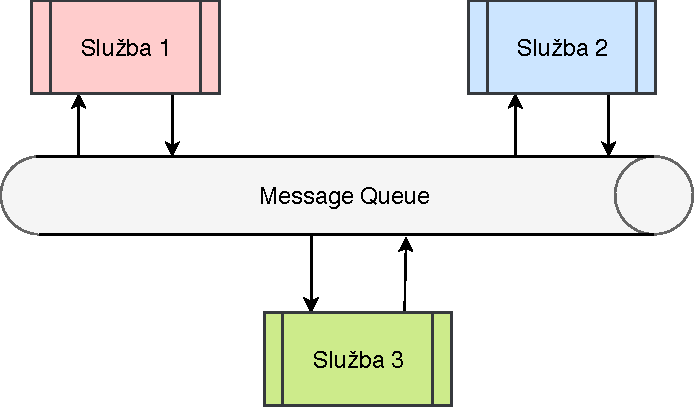
\includegraphics[keepaspectratio=true, width=0.5\linewidth]{figures/message-queue.pdf}
    \caption{Komunikace služeb pomocí Message Queue}
    \label{fig:message-queue}
\end{figure}

Dalším z konceptů, který v rámci SOA vznikl, jsou tzv. \textit{Message Queue} (MQ).
Základní myšlenkou MQ, znázorněnou na obrázku~\ref{fig:message-queue},
je asynchronní komunikace služeb pomocí zpráv nezávislých
na platformě. Komunikaci zprostředkovává fronta, která přijímá a rozesílá
zprávy mezi službami. To přináší vyšší škálovatelnost a menší provázanost
mezi službami. Všechny služby ale musí používat jednotný formát zpráv.

MQ přináší dva způsoby, kterými mohou služby komunikovat. Prvním je
\textit{Request/Reply}, připomínající konverzaci dvou lidí. Jedna
služba zašle zprávu obsahující identifikátor konverzace. Druhá služba
na obdrženou zprávu zašle odpověď a pomocí identifikátoru označí,
ke které otázce odpověď patří. Druhým způsobem je \textit{publish-subscribe},
kdy existuje více front s různými tématy (\textit{topics}) a služby mohou
do těchto front přispívat relevantními zprávami nebo je konzumovat jako odběratelé.

\subsection{Enterprise Service Bus}

Ačkoliv zmíněné modely usnaďnují komunikaci služeb a zvyšují jejich
spolehlivost, integrace služeb může být obtížná kvůli různým
komunikačním protokolům a formátům. Již v devadesátých letech
byl představen koncept \textit{Enterprise Service
Bus} (ESB)~\cite{chappell2004enterprise},
znázorněný na obrázku~\ref{fig:enterprise-service-bus},
který má za úkol propojit heterogenní služby a zajistit mezi nimi
komunikační kanály. Tím na sebe ESB přebírá zodpovědnost za překlad
jednotlivých zpráv a centralizuje veškerou komunikaci v systému.

ESB se zároveň staví do role experta na lokalizaci jednotlivých služeb.
Službě tak pro komunikaci s okolním světem stačí znát adresu ESB, kterému
zašle zprávu, a ten ji sám doručí na místo určení. Tento model ale
znamená, že ESB je velmi komplexní komponentou. Výpadek ESB navíc
v způsobí zastavení funkce celého systému a ESB se tak stává
tzv. \textit{single point of failure}, což v praxi snižuje škálovatelnost systému.
V případě vlastního nízkého výkonu se ESB může snadno stát úzkým hrdlem.
Tyto problémy mohou být částečně vyřešeny tzv. \textit{federovaným designem},
kdy je systém rozdělen na byznysově příbuzné části, z nichž každá má
svůj ESB.

\begin{figure}
    \centering
    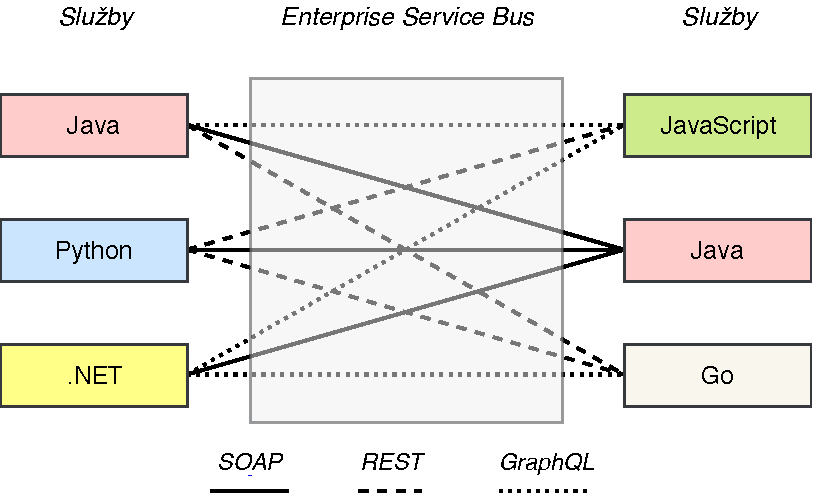
\includegraphics[keepaspectratio=true, width=0.7\linewidth]{figures/enterprise-service-bus.pdf}
    \caption{Komunikace služeb skrz Enterprise Service Bus}
    \label{fig:enterprise-service-bus}
\end{figure}

\subsection{Microservices}

\goal{Microservices a budoucnost SOA}
Novým trendem posledních let jsou takzvané \textit{Microservices}.
Přináší několik zajmavých konceptů, které specializují a konkretizují
principy SOA. Microservices se tedy dají chápat jako podmnožina
SOA. Základní myšlenkou je vývoj informačního systému jako množiny
malých oddělených služeb, které jsou spouštěny v samostatných procesech
a komunikují spolu pomocí jednoduchých protokolů~\cite{lewis2014microservices}.

\goal{Stavba služeb kolem byznysových schopností}
Důležitou myšlenkou microservices je organizace služeb kolem
byznysových schopností systému. Namísto horizontálního dělení monolitu
podle jeho vrstev\footnote{
Zde předpokládáme klasickou třívrstvou architekturu~\cite{fowler2002patterns},
rozdělující systém na \textit{datovou vrstvu}, \textit{aplikační vrstvu}
a \textit{prezentační vrstvu}. Tyto vrstvy mají oddělené zodpovědnosti a komunikují
spolu pomocí jasně definovaných společných rozhraní.
} navrhuje rozdělit monolit vertikálně podle jeho byznysových schopností.
Na obrázku~\ref{fig:monolith-vs-microservices} je toto rozdělení demonstrováno.
Příkladem může být dělení e-commerce systému na jednu službu obsahující byznysovou
logiku pro registraci a správu uživatelů, druhou službu obsahující byznysovou logiku
pro práci s produkty a třetí službu obsahující byznysovou logiku pro práci
s objednávkami.

\begin{figure}
    \centering
    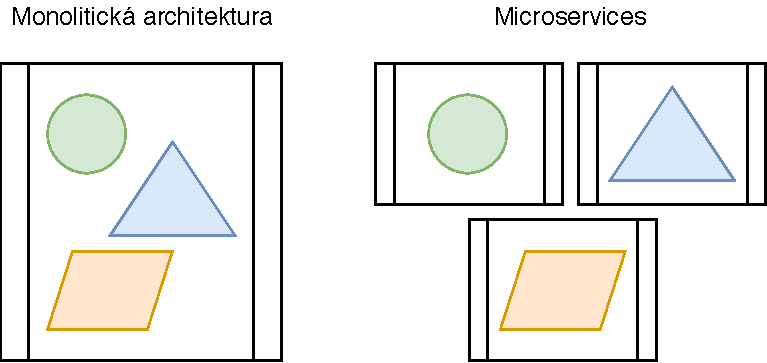
\includegraphics[keepaspectratio=true, width=0.5\linewidth]{figures/monolith-vs-microservices.pdf}
    \caption{Porovnání struktury monolitické architektury a microservices}
    \label{fig:monolith-vs-microservices}
\end{figure}

\goal{Myšlenka nahraditelnosti komponenty}
Koncept microservices přemýšlí o službě jako o samostatné komponentě,
kterou lze individuálně vyměnit či vylepšit, bez nutnosti zásahu do
ostatních služeb~\cite{lewis2014microservices}. Monolitická architektura
vyžaduje i při malé změně jedné části celý systém znovu zkompilovat, sestavit
a nasadit. Malé služby sloužící ideálně jedinému byznysovému účelu lze naopak
při změně byznysových požadavků snadno nahradit samostatně bez zásahu do zbytku
systému. Tím se usnaďnuje cyklus nasazení a spuštění nové verze služby.

\goal{Myšlenka smart endpoints, dumb pipes}
Microservices také přinášejí koncept \uv{smart endpoint, dumb pipes},
který opouští koncept ESB ve prospěch přesunutí veškeré byznys logiky
na stranu služeb. Tím se zvyšuje zapouzdřenost služeb a snižuje se
jejich vzájemné provázání.

\goal{Škálovatelnost}
Další nespornou výhodou je vysoká škálovatelnost systému. Pokud je na
některou ze služeb kladen vyšší nárok na výkon než na ostatní, mají
vývojáři možnost konkrétní službu horizontálně škálovat aniž by
museli škálovat celý systém, na rozdíl od monolitické architektury.
Srovnání přístupů je znázorněno na obrázku~\ref{fig:microservices-deployment}.
Tím se snižují nároky na systémové zdroje.

~\cite{perrey2003service}
~\cite{sprott2004understanding}

\goal{Distribuce }
% TODO: dopsat

\goal{Four tier architecture}
~\cite{nginx2015fourtier}
% TODO: dopsat nebo zahodit

\goal{Service discovery}
% TODO: dopsat

\goal{Service orchestration & choreography}
% TODO: dopsat

\goal{Definice služby}
\paragraph{Definice: Služba} je ucelenou systémovou komponentou
s jasně definovanou zodpovědností, kterou lze nasadit a spustit jako
samostatný proces, a která komunikuje s ostatními službami pomocí zpráv.

\begin{figure}
    \centering
    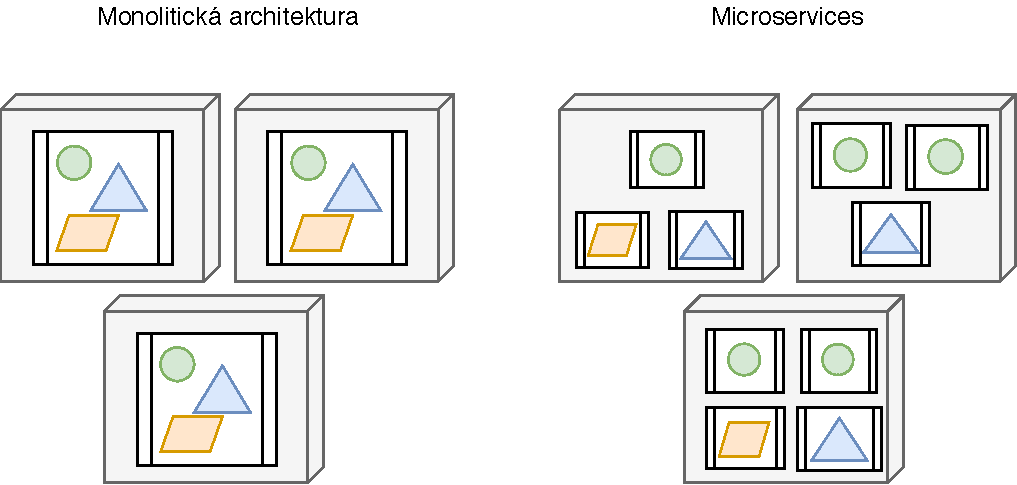
\includegraphics[keepaspectratio=true, width=0.8\linewidth]{figures/microservices-deployment.pdf}
    \caption{Porovnání nasazení monolitické architektury a microservices}
    \label{fig:microservices-deployment}
\end{figure}

\section{Nedostatky současného přístupu}

\goal{Navázání na předchozí sekci}
Jak jsme zjistili v předchozích odstavcích, SOA se zaměřuje zejména na
dělení systému na služby a detailně rozebírá formu jejich vzájemné komunikace.
Neodpovídá ale na několik závažných otázek, se kterými se v praxi musejí
architekti informačních systémů vypořádat, aby architektura byla schopná uspokojivě
plnit požadavky, které jsou na ní kladené.

\goal{Problémy SOA a průřezových problémů}
Jelikož jedním z cílů SOA, potažmo microservices, je co nejvíce izolovat
jednotlivé služby, mají tyto architektury tendenci duplikovat části kódu
zajišťující funkcionalitu, která vyžaduje konzistentní zpracování ve více
službách~\cite{cerny2017disambiguation}, tzv. \textit{průřezových
problémů} (z anglického \textit{cross-cutting concerns}).
Příkladem mohou být právě byznysová pravidla~\cite{cemus2014aspect}, která je potřeba
zohlednit v rámci různých byznysových kontextů realizovaných ve více službách.
Mezi další příklady se řadí logování, monitoring či sběr dat
o telemetrii procesů.

\goal{Nastínění konkrétního příkladu}
Abychom si mohli lépe představit diskutovaný problém, znázorněmě
si ho na konkrétním příkladu. Uvažme e-commerce systém
skládající se z několika služeb naprogramovaných v různých technologiích,
organizovaných kolem jeho byznysových funkcí.
Jedna služba obsluhuje byznysové operace vázající
se na uživatele systému, jejich registraci a administraci. Druhá
služba realizuje operace s produkty, jejich vytváření, úpravu,
správu skladových zásob a informace o dostupnosti. Třetí služba je
zodpovědná za vytváření a správu objednávek, informování uživatelů
o změnách jejich stavů a vytváření statistik a reportů pro management.
Čtvrtá služba má na starosti účetnictví, tedy vystavování a přijímání
faktur a komunikaci s bankovními službami o potvrzení přijatých plateb.
Poslední, pátá služba, poskytuje uživatelské rozhraní pro uživatele
systému a umožňuje jeho komfortní obsluhu.

\goal{Konkrétní problémy zpracování průřezových problémů na příkladu}
Jak již víme, každá byznysová operace má své preconditions, které musejí být splněny,
aby mohla být vykonána. Operace má také post-conditions, které musejí být
aplikovány po skončení operace. Například při vytváření faktury za
objednávku musí být zvalidována fakturační adresa, bez níž nemůže
být faktura vystavena. Pokud chceme ušetřit práci účetníkům, kteří by
v případě nevalidní adresy musely kontaktovat zákazníka – pokud vůbec
takovou možnost mají – musíme tento fakt je zohlednit již při vytváření objednávky.
Proces vytváření objednávky ale realizuje jiná služba než vystavování faktur.
V ideálním případě bychom chtěli zákazníka upozornit na nevalidní fakturační
adresu dynamicky ještě před odesláním objednávkového formuláře přímo v uživatelském
rozhraní~\cite{cemus2017separation}. Pro lepší představu je problém znázorněn na
obrázku~\ref{fig:service-cutting},

\goal{Náročná reakce na změnu požadavku}
Z tohoto příkladu je jasně vidět, že stejná funkcionalita se promítá
do tří služeb, z nichž každá má zodpovědnost za jiné byznysové operace. Ve chvíli,
kdy vzejde požadavek na změnu validace fakturační adresy – řekněme, že chceme zobecnit
validaci PSČ a umožníme přijímat i jeho tvar s mezerou – musíme stejnou změnu
provést konzistentně na třech různých místech, všechny tři služby znovu
sestavit a nasadit ve správném pořadí tak, aby nedošlo ke stavu,
kdy jedna služba přijme nový tvar PSČ, ale navazující služba ho není
schopna zpracovat.

\goal{Microservices neříká nic o tom, jak velké je mikro}
Pozorný čtenář může namítnout, že problém validace fakturačních adres by
bylo možné vyřešit vyčleněním této funkcionality
do samostatné služby a vystavit její rozhraní pro ostatní služby,
v souladu s nosnou myšlenkou microservices. Je pravda, že microservices
v názvu nese slovo \uv{micro} a evokuje tak, že služby by měly být co nejmenší
a nést co nejméně zodpovědnosti. Může ale nastat stav, kdy je služba příliš malá?

\goal{Nevýhody příliš malé služby}
Pokud služby ponesou příliš málo odpovědnosti,
přináší to s sebou několik problémů, které je nutné zvážit. Musíme mít na paměti, že
nasazení a provoz každé služby s sebou přináší náklady navíc
a zvyšuje časové nároky na jejich vývojáře a administrátory.
Komunikace služeb po síti je navíc podstatně pomalejší a náchylnější na
chybu než komunikace jednotlivých komponent v rámci jednoho procesu.
S rostoucím počtem \textit{průřezových problémů} by tak i rychle rostl
počet služeb v systému a celkové náklady na jeho vývoj a údržbu.

\begin{figure}
    \centering
    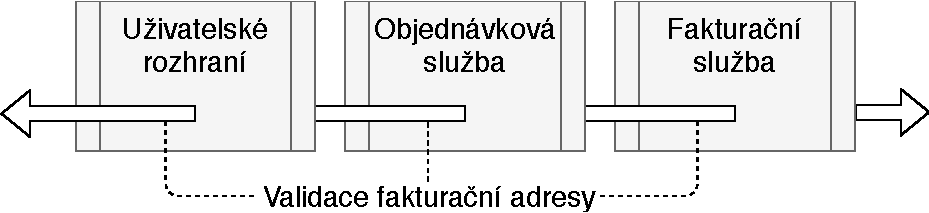
\includegraphics[keepaspectratio=true, width=0.8\linewidth]{figures/service-cutting.pdf}
    \caption{Příklad zásahu jedné funkcionality do více služeb}
    \label{fig:service-cutting}
\end{figure}

\goal{Shrnutí problémů}
Na příkladu můžeme vidět, že existuje typ problémů, které v rámci architektury
orientované na služby při využití současného přístupu nejsme schopni uspokojivě
vyřešit na jednom místě a vedou k duplikaci znalostí na více místech systému.
Taková duplikace může vést k zvýšenému riziku lidské chyby vývojáře a tím k
nekonzistentnímu chování systému. Navíc zvyšuje cenu na vývoj a údržbu systému.

\section{Identifikace požadavků na implementaci frameworku}

Z příkladu popsaného výše můžeme identifikovat požadavky, které by měly
být zohledněny při návrhu a implementaci frameworku, který bude sloužit
pro centrální administraci a automatickou distribuci byznysových pravidel
v architektuře orientované na služby.

Framework, resp. jeho knihovny, by měly umožňovat:

\begin{itemize}
    \item{Definice byznys kontextů pomocí doménově specifického jazyka srozumitelného pro doménové experty}
    \item{Zápis preconditions a post-conditions pravidla jednotlivých byznys kontextů}
    \item{Možnost jednoho kontextu rozšiřovat jiné kontexty}
    \item{Možnost centrálně spravovat byznysové kontexty, včetně úpravy stávajících a vytváření nových kontextů}
    \item{Automatická distribuce kontextů, vyhodnocování jejich preconditions a aplikace post-conditions}
\end{itemize}

\section{Shrnutí}

V této kapitole jsme nastínili problematiku vysoké komplexity moderních informačních systémů
a z toho vyplívající požadavky na jejich architekturu. Analyzovali jsme koncept byznysových
pravidel a byznysových kontextů. Dále jsme zkomali architekturu orientovanou na služby, její
výhody a nevýhody, její moderní evoluci v podobě microservices a identifikovali jsme problémy
v souvislosti s průřezovými problémy, které zasahují do více služeb najednou. Nakonec jsme
vyjmenovali požadavky, které by měl splňovat framework, který bude výstupem této práce.
